\documentclass[12pt,a4paper]{article}

\usepackage[utf8]{inputenc}
\usepackage[T1]{fontenc}
\usepackage[spanish,es-nodecimaldot]{babel}
\usepackage{csquotes}
\usepackage[margin=2.5cm]{geometry}
\usepackage{setspace}
\usepackage{graphicx}
\usepackage{booktabs}
\usepackage{array}
\usepackage{longtable}
\usepackage{newunicodechar}
\newunicodechar{̇}{}
\usepackage{hyperref}
\usepackage{float}
\usepackage[backend=biber,style=ieee,sorting=none]{biblatex}

\addbibresource{referencias.bib}

\onehalfspacing
\hypersetup{hidelinks}

\begin{document}

% ===================== CARÁTULA =====================
\thispagestyle{empty}
\begin{center}
\vspace*{1.5cm}

{\fontsize{22}{26}\selectfont\bfseries UNIVERSIDAD TÉCNICA ESTATAL\\[4pt] DE QUEVEDO\par}

\vspace{1.4cm}

{\large\bfseries FACULTAD DE CIENCIAS DE LA COMPUTACIÓN\par}

\vspace{1.2cm}

{\small\itshape CARRERA DE INGENIERÍA EN SOFTWARE\par}

\vspace{1.2cm}

{\large\bfseries ASIGNATURA:\par}
{\large Aplicaciones Distribuidas\par}

{\large\bfseries TEMA:\par}
\vspace{0.4cm}
{\large\bfseries Informe Académico Individual: Análisis Crítico Comparativo de Elasticsearch y Apache Solr como Sistemas Distribuidos\par}

\vspace{1.0cm}

{\large\bfseries PRESENTADO POR:\par}
\vspace{2pt}
{\large HERRERA BARCO HUMBERTO ALDAIR\par}

\vspace{1.0cm}

{\large\bfseries FECHA:\par}
{\large 13/11/2026\par}

\end{center}

\newpage
\tableofcontents
\newpage

% ===================== RESUMEN =====================
\section*{Resumen}
\addcontentsline{toc}{section}{Resumen}

Este informe analiza críticamente a Elasticsearch como sistema distribuido real y lo compara con Apache Solr (SolrCloud), un motor de búsqueda y análisis basado en Apache Lucene que resuelve problemas similares de indexación y consulta de grandes volúmenes de información. El estudio aplica conceptos de la Unidad 1: transparencias de distribución, teorema CAP y extensión PACELC, modelos de comunicación y tolerancia a fallos. La metodología combina la revisión de artículos académicos recientes y documentación técnica oficial con una experimentación propia sobre un clúster local de Elasticsearch de tres nodos desplegado con Docker Compose. Durante las pruebas se creó un índice con tres shards primarios y una réplica, se verificó la distribución de fragmentos y se evaluó el comportamiento ante la caída y recuperación del nodo \texttt{es02}. Los resultados mostraron que el clúster mantuvo el estado \textit{green} y conservó los shards activos mediante la reasignación entre los nodos disponibles, evidenciando mecanismos de replicación y recuperación. La comparación con SolrCloud permitió identificar similitudes arquitectónicas y diferencias en la gestión de réplicas, coordinación y compromisos de consistencia, disponibilidad y latencia. Se concluye que Elasticsearch ofrece una solución distribuida adecuada para búsqueda y análisis escalables, aunque su operación exige comprender sus configuraciones y límites ante particiones y fallos.

% ===================== INTRODUCCIÓN =====================
\section{Introducción}

\subsection{Problema que resuelve el sistema}
El crecimiento del volumen de datos textuales y estructurados ha hecho necesario contar con sistemas capaces de indexar y buscar información de forma eficiente. Elasticsearch es un motor de búsqueda y análisis distribuido orientado al almacenamiento, indexación y consulta de grandes volúmenes de datos, lo que lo hace útil en escenarios como búsqueda de texto completo, análisis de registros y observación de plataformas \cite{cheresharov-2026,calderon-2023,feraru-2026}. Apache Solr es una alternativa basada también en Apache Lucene, ampliamente utilizada para búsqueda e indexación distribuida; su uso en casos reales y estudios comparativos permite contrastar capacidades y decisiones de diseño frente a Elasticsearch \cite{deniz-2023,lu-2026,unger-2023}.

\subsection{Uso y escala}
Elasticsearch se emplea en aplicaciones donde se requiere consultar y analizar datos de manera rápida sobre conjuntos distribuidos, apoyándose en una arquitectura de clúster que permite escalar horizontalmente mediante nodos y partición de índices en shards \cite{elastic_distributed_architecture,elastic_nodes_shards,calderon-2023}. En el caso de Solr, su modo distribuido (SolrCloud) permite repartir colecciones en shards y réplicas para atender cargas de búsqueda e indexación \cite{solr_shards_indexing,deniz-2023}. La elección de uno u otro sistema depende de factores como el tipo de carga, los requisitos de consistencia, la tolerancia a fallos, el rendimiento y la operación del clúster.

\subsection{Motivación de la elección}
Se eligió Elasticsearch por la posibilidad de desplegar un clúster local con Docker Compose y observar de manera práctica conceptos de sistemas distribuidos: formación del clúster, partición de datos en shards, replicación, y reacción ante la caída y recuperación de un nodo. La comparación con Apache Solr se consideró pertinente porque ambos resuelven el problema de la búsqueda distribuida y permiten analizar compromisos de diseño distintos dentro del mismo dominio \cite{deniz-2023}.

% ===================== ARQUITECTURA =====================
\section{Arquitectura del sistema}

\subsection{Componentes principales de Elasticsearch}
Un clúster de Elasticsearch está compuesto por uno o más nodos, donde cada nodo es una instancia del servidor que participa en el almacenamiento de datos y en la ejecución de operaciones de indexación y búsqueda \cite{elastic_nodes_shards,elastic_distributed_architecture}. Los datos se organizan en índices, y cada índice se divide en shards. Los shards primarios contienen la partición original de los datos, mientras que las réplicas son copias de esos shards que aportan redundancia y pueden contribuir a la disponibilidad y al procesamiento de consultas \cite{elastic_nodes_shards,elastic_read_write}.

Los nodos pueden desempeñar distintos roles (por ejemplo, maestro, de datos, de ingesta o coordinadores), lo que permite separar responsabilidades dentro del clúster \cite{elastic_nodes_shards}. En el experimento realizado se desplegaron tres nodos (\texttt{es01}, \texttt{es02} y \texttt{es03}) que conformaron un clúster funcional, lo cual permitió observar la distribución de shards y la respuesta ante fallos.

\subsection{Comunicación entre componentes}
Los clientes interactúan con Elasticsearch principalmente mediante su API REST sobre HTTP, mientras que los nodos se comunican internamente a través de la capa de transporte del clúster \cite{elastic_distributed_architecture}. Cuando un cliente envía una solicitud, el nodo que la recibe puede actuar como nodo coordinador: determina qué shards deben participar, reenvía la operación a los nodos correspondientes y combina los resultados antes de responder \cite{elastic_read_write,elastic_distributed_architecture}.

En las operaciones de escritura, la solicitud se dirige al shard primario correspondiente y luego se replica a las réplicas del shard, lo que implica coordinación entre nodos para mantener las copias actualizadas \cite{elastic_read_write}. En las búsquedas, el sistema puede consultar copias del shard (primaria o réplicas), lo que favorece la distribución de la carga. Este modelo refleja una comunicación cliente-servidor hacia el clúster y una coordinación interna entre nodos para ejecutar operaciones distribuidas.

\subsection{Componentes principales de Apache Solr (SolrCloud)}
En SolrCloud, los datos se organizan en colecciones que se dividen en shards, y cada shard puede tener múltiples réplicas. Una réplica actúa como líder del shard y coordina las actualizaciones, mientras que las demás réplicas mantienen copias del índice según su tipo \cite{solr_shards_indexing}. SolrCloud soporta distintos tipos de réplicas (NRT, TLOG y PULL), que ofrecen diferentes compromisos entre capacidad de liderazgo, actualización y costo de recuperación \cite{solr_shards_indexing,solr_recoveries}.

Las solicitudes distribuidas se enrutan a través del clúster para alcanzar los shards necesarios, y el sistema incorpora mecanismos para balanceo y tolerancia ante fallos en la atención de consultas \cite{solr_distributed_requests}. Esta arquitectura lo hace comparable con Elasticsearch en términos de partición, replicación y coordinación distribuida.

\subsection{Diagrama de arquitectura}
\begin{figure}[H]
    \centering
    \IfFileExists{figuras/arquitectura_elasticsearch.png}{
        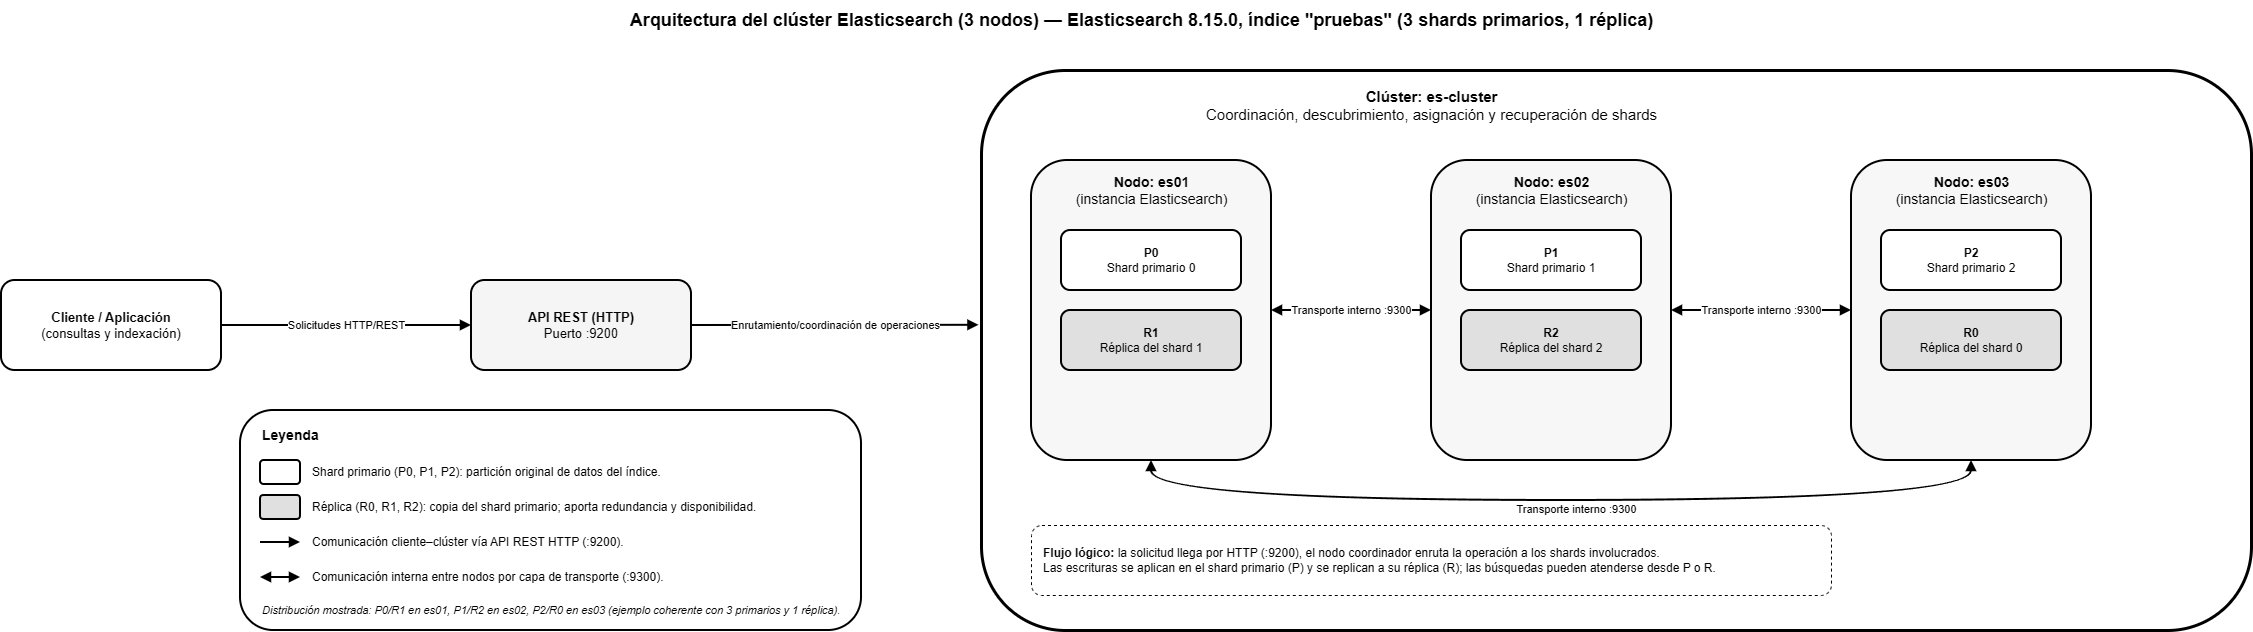
\includegraphics[width=0.88\textwidth]{figuras/arquitectura_elasticsearch.png}
    }{
        \fbox{\parbox[c][6cm][c]{0.88\textwidth}{\centering Agregar el diagrama propio en \texttt{figuras/arquitectura\_elasticsearch.png} (exportado desde draw.io).}}
    }
    \caption{Arquitectura del clúster de Elasticsearch analizado (elaboración propia).}
    \label{fig:arquitectura}
\end{figure}

\subsection{Evolución desde el esquema a mano (Anexo A)}
El diagrama final se basó en un boceto inicial elaborado a mano (Anexo~\ref{anexo:esquema}). A partir de ese esquema se precisaron los elementos del clúster observados en la práctica: el cliente, el acceso HTTP al clúster, los tres nodos (\texttt{es01}, \texttt{es02} y \texttt{es03}), la distribución de shards primarios y réplicas, y la comunicación interna de transporte entre nodos. Esta evolución permitió pasar de una representación general a un diagrama más alineado con la arquitectura desplegada y analizada en la experimentación.

% ===================== ANÁLISIS UNIDAD 1 =====================
\section{Análisis con los conceptos de la Unidad 1}

\subsection{Transparencias de distribución}
Las transparencias de distribución ocultan aspectos de la naturaleza distribuida del sistema. A partir de la documentación oficial y de la experimentación realizada, se puede analizar su presencia en Elasticsearch y contrastarla con SolrCloud.

\begin{itemize}
    \item \textbf{Transparencia de acceso:} Elasticsearch expone una interfaz HTTP/REST para interactuar con índices y documentos, lo que ofrece una forma uniforme de acceso para los clientes \cite{elastic_distributed_architecture,elastic_read_write}. En SolrCloud, las operaciones también se realizan mediante interfaces HTTP sobre colecciones y shards distribuidos \cite{solr_distributed_requests,solr_shards_indexing}.
    \item \textbf{Transparencia de ubicación:} el cliente no necesita conocer en qué nodo específico se encuentra cada shard para realizar una consulta o indexación, ya que el clúster coordina el enrutamiento y la ejecución distribuida \cite{elastic_read_write,solr_distributed_requests}. Sin embargo, la ubicación física/lógica sigue siendo relevante para la administración del clúster.
    \item \textbf{Transparencia de migración:} los shards pueden reasignarse entre nodos (por ejemplo, ante cambios en el clúster o recuperación), lo que permite mover datos sin que el cliente gestione manualmente cada movimiento \cite{elastic_nodes_shards,elastic_resilience,solr_recoveries}.
    \item \textbf{Transparencia de reubicación:} la reubicación de shards durante la operación del clúster es posible como parte de la gestión y recuperación, aunque puede tener impacto en rendimiento y estado del clúster; por ello, no es completamente invisible desde el punto de vista operativo \cite{elastic_resilience,solr_recoveries}.
    \item \textbf{Transparencia de replicación:} Elasticsearch utiliza réplicas de shards para redundancia y soporte de disponibilidad/consultas \cite{elastic_nodes_shards,elastic_read_write}. SolrCloud también emplea réplicas por shard, con tipos que definen su comportamiento y capacidad de liderazgo \cite{solr_shards_indexing}. La replicación existe y aporta beneficios, aunque su configuración no es transparente para el administrador.
    \item \textbf{Transparencia de concurrencia:} múltiples clientes pueden operar sobre el sistema distribuido; el control de concurrencia y la coordinación de escrituras/lecturas se gestionan internamente en los mecanismos de shard primario, replicación y coordinación \cite{elastic_read_write,solr_shards_indexing}. No obstante, el comportamiento bajo concurrencia depende de la configuración y del tipo de operación.
    \item \textbf{Transparencia de fallos:} ambos sistemas incorporan mecanismos para tolerar fallos (réplicas, elección/gestión de líderes y recuperación), lo que puede ocultar ciertos fallos al cliente \cite{elastic_resilience,solr_distributed_requests,solr_recoveries}. En el experimento, la caída de \texttt{es02} no impidió que el clúster mantuviera shards activos, aunque el evento sí fue observable a nivel administrativo.
\end{itemize}

\subsection{Teorema CAP y extensión PACELC}

\subsubsection{Comportamiento ante partición de red (CAP)}
Ante una partición de red, un sistema distribuido debe enfrentar el compromiso entre consistencia y disponibilidad. En Elasticsearch, la disponibilidad y la integridad del clúster dependen de mecanismos como el descubrimiento de nodos, la elección de nodo maestro y las reglas de asignación/recuperación de shards; configuraciones inadecuadas o la pérdida de quórum pueden afectar la capacidad del clúster para operar correctamente \cite{elastic_discovery,elastic_resilience}. En SolrCloud, la coordinación del clúster y la gestión de líderes/réplicas también influyen en el comportamiento ante fallos y particiones, y los procesos de recuperación buscan restablecer el estado operativo de los shards \cite{solr_shards_indexing,solr_recoveries,solr_distributed_requests}.

En términos prácticos, tanto Elasticsearch como SolrCloud priorizan la continuidad operativa mediante replicación y mecanismos de recuperación, pero el resultado ante una partición depende de la configuración, del número de nodos elegibles y del estado de las réplicas. Por ello, la clasificación CAP no debe asumirse de forma simplista sin considerar la configuración específica del clúster \cite{elastic_resilience,solr_recoveries}.

\subsubsection{Comportamiento sin partición (PACELC)}
Cuando no existe partición, el compromiso se desplaza hacia latencia y consistencia. En Elasticsearch, las operaciones de escritura se procesan en el shard primario y se propagan a las réplicas, lo que introduce coordinación y posibles costos de latencia según la configuración y el estado del clúster \cite{elastic_read_write,elastic_resilience}. En búsquedas, la posibilidad de consultar réplicas puede favorecer la distribución de carga y la latencia de respuesta.

En SolrCloud, los tipos de réplica (NRT, TLOG y PULL) implican diferentes equilibrios: algunas réplicas pueden participar en liderazgo y mantener información para recuperación, mientras que otras priorizan la reducción de costo de indexación local a cambio de mayor dependencia de la replicación desde el líder \cite{solr_shards_indexing,solr_recoveries}. Esto muestra un compromiso entre latencia, frescura de datos y complejidad de recuperación, coherente con el enfoque de PACELC.

\subsection{Modelos de comunicación}
El modelo predominante en la interacción externa es **cliente-servidor**: los clientes envían solicitudes al clúster (Elasticsearch o SolrCloud) y reciben respuestas a través de interfaces HTTP \cite{elastic_distributed_architecture,solr_distributed_requests}. Internamente, la comunicación se da entre nodos del clúster para coordinar descubrimiento, elección de roles/liderazgo, enrutamiento de solicitudes, replicación y recuperación \cite{elastic_discovery,elastic_read_write,solr_shards_indexing,solr_recoveries}.

Respecto al modo de comunicación, las solicitudes cliente-clúster suelen manejarse como interacciones petición-respuesta; sin embargo, dentro del clúster existen procesos coordinados que pueden involucrar esperas y confirmaciones (por ejemplo, propagación de escrituras o procesos de recuperación) según la operación y configuración \cite{elastic_read_write,solr_recoveries}. Por ello, el sistema combina un acceso externo tipo cliente-servidor con mecanismos internos de coordinación distribuida.

\subsection{Tolerancia a fallos}

\subsubsection{Fallos soportados, detección y recuperación}
En Elasticsearch, la tolerancia a fallos se apoya en la replicación de shards y en los mecanismos de gestión del clúster. La elección y estabilidad del nodo maestro, el descubrimiento de nodos y la asignación de shards son elementos clave para detectar cambios en la membresía del clúster y responder ante fallos \cite{elastic_discovery,elastic_nodes_shards,elastic_resilience}. Cuando un nodo deja de estar disponible, el clúster puede reasignar réplicas o promover copias para mantener la disponibilidad de los shards, dependiendo de la configuración y del número de réplicas existentes.

En SolrCloud, la tolerancia a fallos se relaciona con la gestión de líderes de shard, la replicación y los procesos de recuperación. Los distintos tipos de réplicas (NRT, TLOG y PULL) influyen en la capacidad de asumir liderazgo y en la forma de recuperarse tras una falla \cite{solr_shards_indexing,solr_recoveries}. Además, la distribución de solicitudes permite continuar atendiendo consultas mientras existan réplicas disponibles \cite{solr_distributed_requests}.

\subsubsection{Evidencia desde la experimentación}
En la prueba realizada, el clúster de tres nodos mantuvo el estado \textit{green} tras la detención de \texttt{es02}, con 2 nodos activos y 6 shards activos (0 sin asignar). Esto indica que las copias necesarias estaban disponibles en los nodos restantes. Al reiniciar \texttt{es02}, el nodo se reincorporó y el clúster redistribuyó shards, recuperando la distribución entre los tres nodos. Esta observación es consistente con el uso de réplicas y reasignación automática como mecanismos de tolerancia a fallos \cite{elastic_nodes_shards,elastic_resilience}.

\subsubsection{Incidente real documentado}
Un caso real documentado es el incidente de Elastic Cloud ocurrido el 18 de enero de 2019 en la región AWS \texttt{eu-west-1}, reportado por Elastic. Según el informe, una alta carga en la capa de coordinación (ZooKeeper) y problemas en la reconexión/caché de clientes del proxy provocaron degradación y, posteriormente, indisponibilidad de los despliegues en la región durante un periodo aproximado de 20 minutos, dentro de un incidente de mayor duración \cite{elastic_cloud_incident_2019}. El reporte describe que la inestabilidad en la coordinación afectó el enrutamiento hacia los clústeres y que la mitigación incluyó estabilizar la capa de coordinación y escalar/ajustar la capa de proxy; además, se plantearon mejoras para reducir el acoplamiento y aumentar la resiliencia. Este incidente ilustra que, en sistemas distribuidos, los fallos o degradaciones en componentes de coordinación y control también pueden impactar la disponibilidad percibida por los usuarios \cite{elastic_cloud_incident_2019,elastic_resilience}.

Como referencia adicional del lado de SolrCloud, el issue \textit{SOLR-7844} documenta un problema en el que la expiración de sesión de ZooKeeper durante la elección de líder de shard podía conducir a múltiples líderes, evidenciando riesgos de coordinación en escenarios de fallo \cite{solr_jira_7844,solr_shards_indexing}.

% ===================== EXPERIMENTACIÓN =====================
\section{Experimentación propia}
\label{sec:experimentacion}

La experimentación se realizó en un clúster local de Elasticsearch 8.15.0 con tres nodos (\texttt{es01}, \texttt{es02}, \texttt{es03}) desplegados mediante Docker Compose. Se ejecutaron pruebas de levantamiento, creación de índice, inserción de documentos, caída de un nodo y recuperación. Los comandos y resultados completos se incluyen en el repositorio.

\subsection{Levantamiento del clúster}
Se iniciaron los contenedores y se verificó el estado del clúster. Los resultados mostraron tres nodos activos, con \texttt{es02} como nodo maestro y estado del clúster \textit{green} (\texttt{number\_of\_nodes: 3}, \texttt{number\_of\_data\_nodes: 3}).

\begin{figure}[H]
    \centering
    \IfFileExists{figuras/captura_01_cluster.png}{
        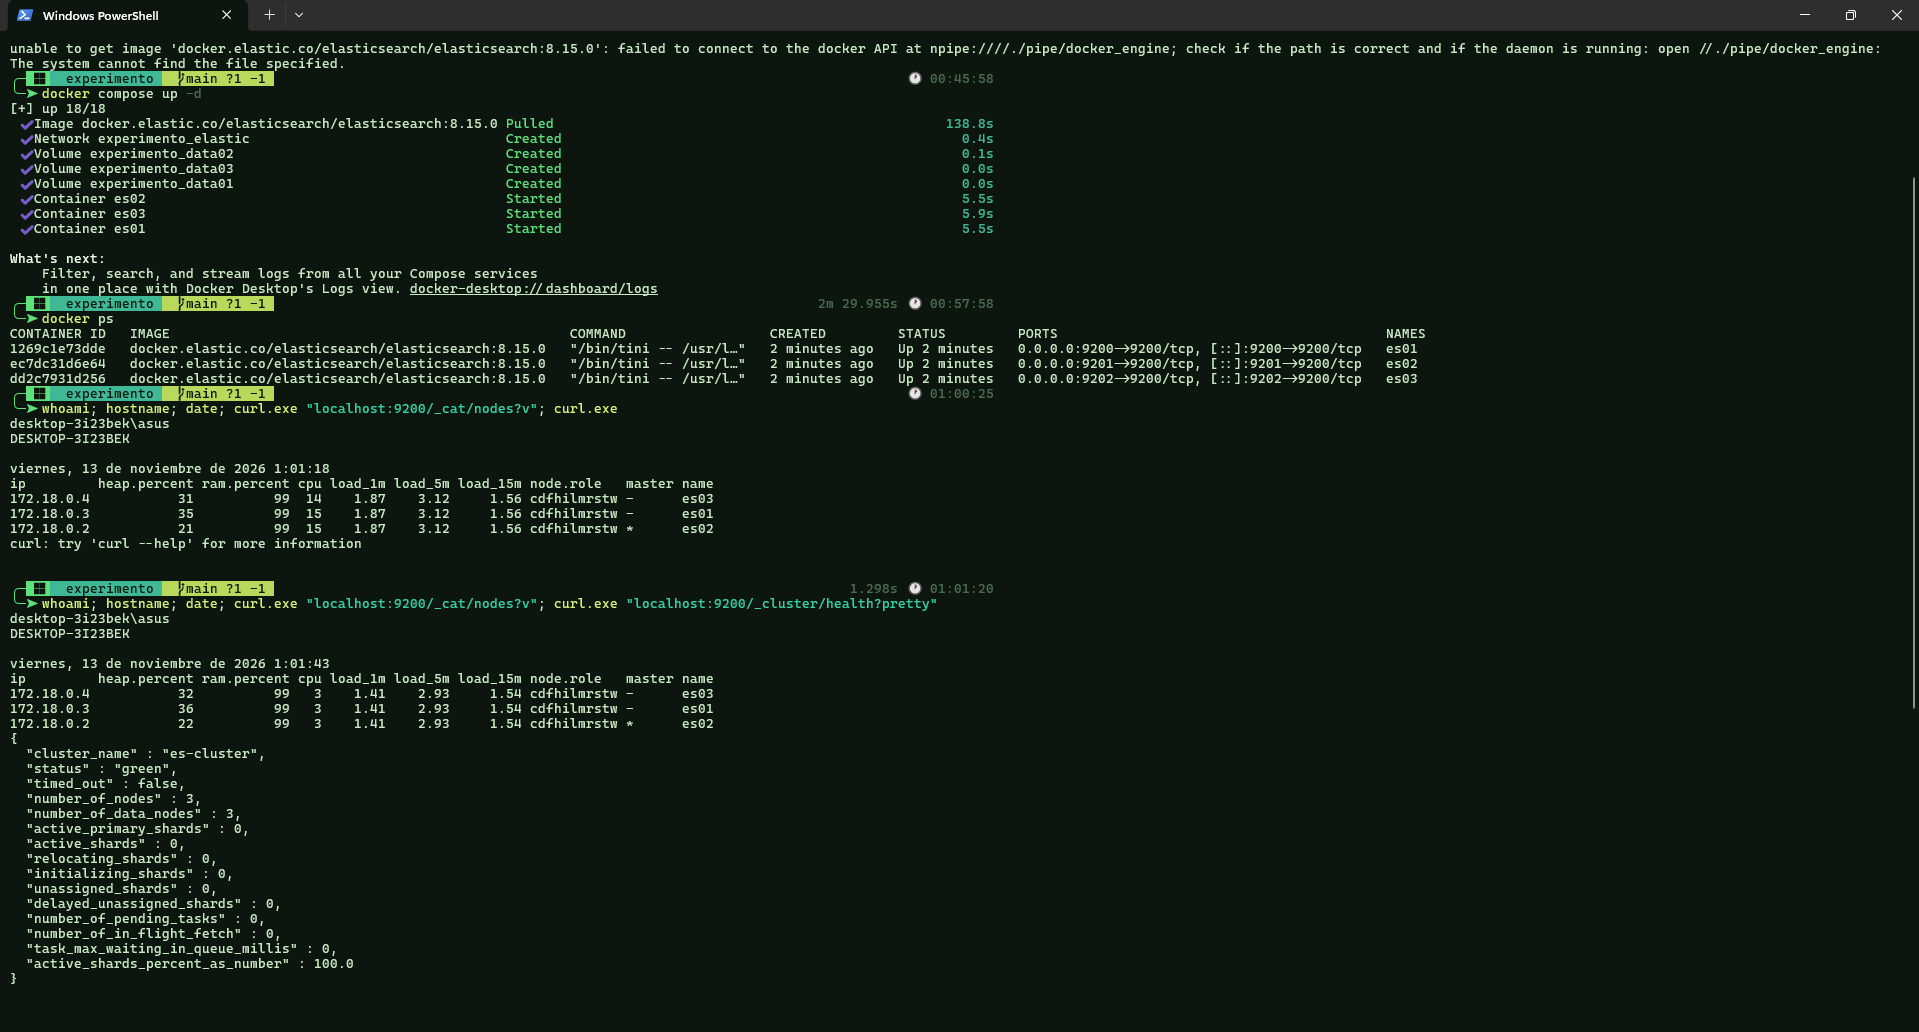
\includegraphics[width=0.92\textwidth]{figuras/captura_01_cluster.png}
    }{
        \fbox{\parbox[c][4cm][c]{0.92\textwidth}{\centering Agregar captura en \texttt{figuras/captura\_01\_cluster.png} (nodos y estado \textit{green}, con usuario/fecha/máquina visibles).}}
    }
    \caption{Levantamiento del clúster de Elasticsearch (captura propia).}
    \label{fig:cluster}
\end{figure}

\noindent\textbf{Interpretación:} El clúster se formó correctamente y alcanzó un estado saludable antes de crear índices. Esto evidencia la capacidad de Elasticsearch para coordinar múltiples nodos como un único sistema distribuido \cite{elastic_distributed_architecture,elastic_discovery}.

\subsection{Creación de índice y distribución de shards}
Se creó el índice \texttt{pruebas} con 3 shards primarios y 1 réplica (\texttt{number\_of\_shards: 3}, \texttt{number\_of\_replicas: 1}), se insertaron 6 documentos y se ejecutó \texttt{\_refresh}. La consulta \texttt{\_cat/shards/pruebas?v} mostró 6 shards en estado \texttt{STARTED} (3 primarios y 3 réplicas), con distribución de documentos entre shards y réplicas ubicadas en nodos distintos a sus primarios.

\begin{figure}[H]
    \centering
    \IfFileExists{figuras/captura_02_shards.png}{
        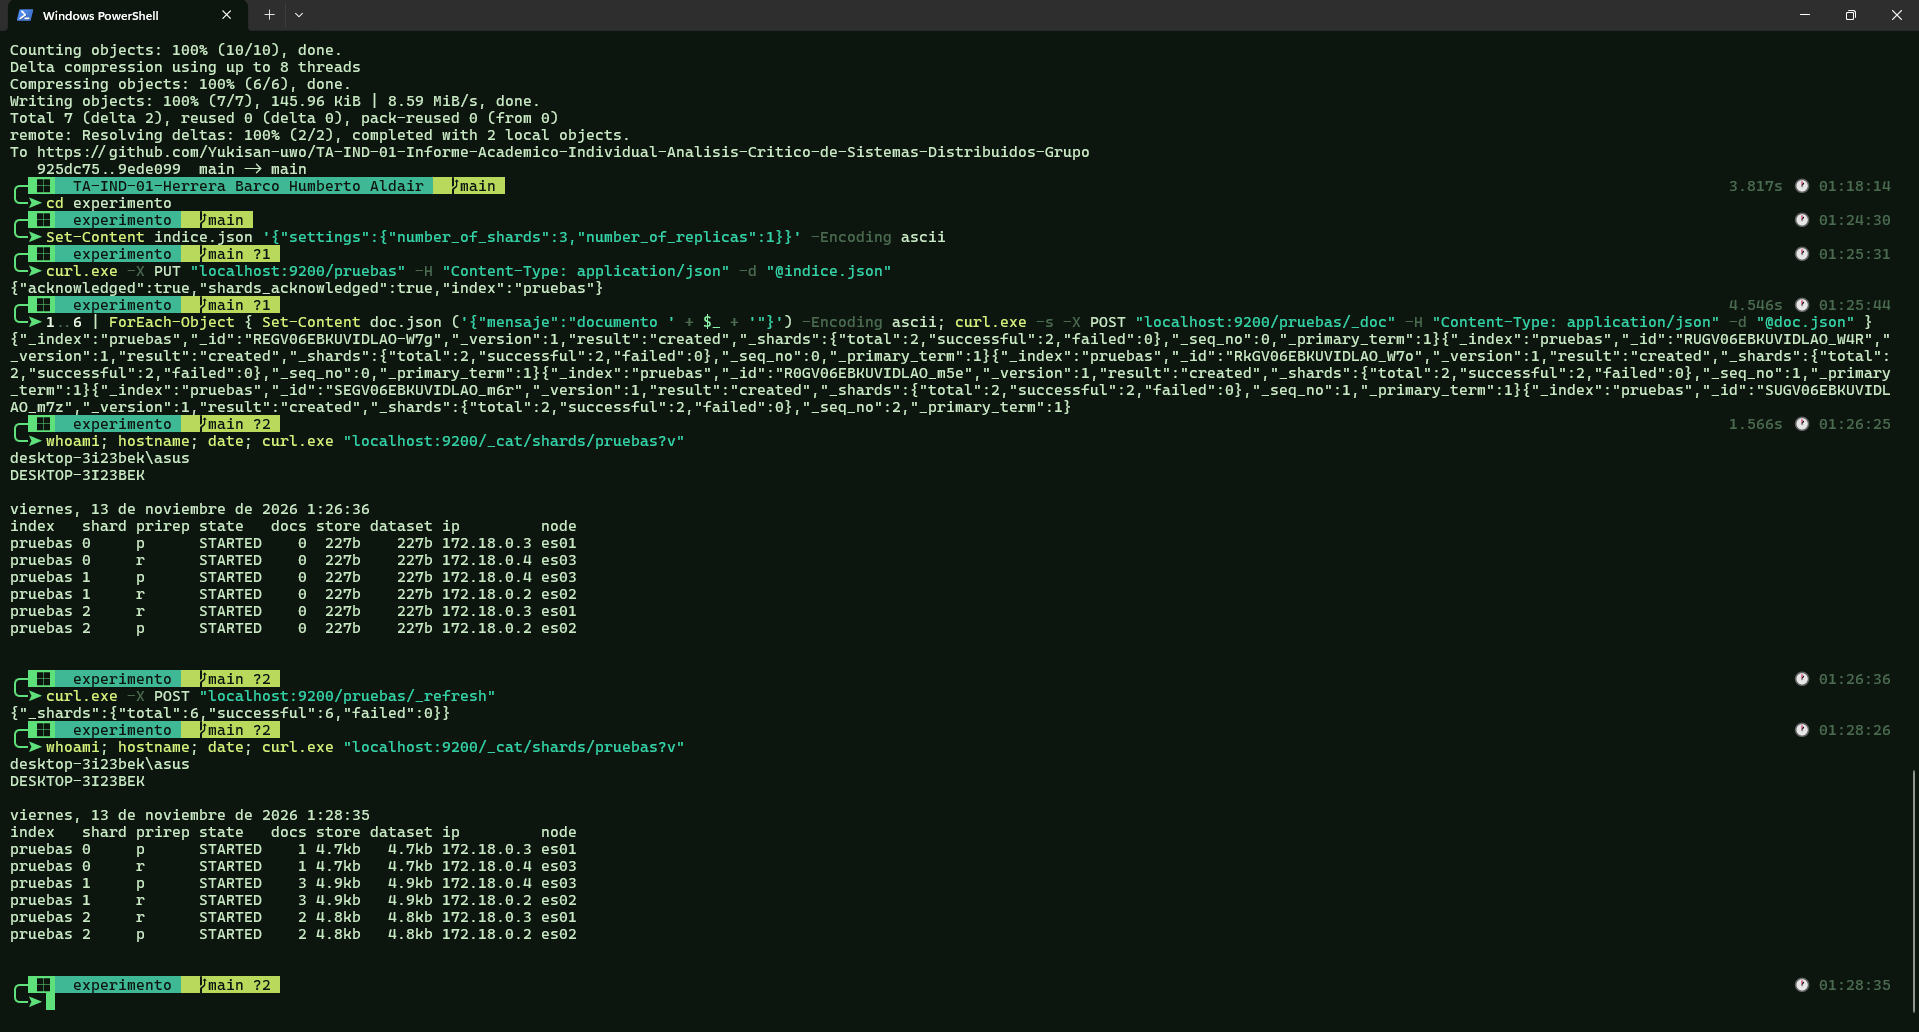
\includegraphics[width=0.92\textwidth]{figuras/captura_02_shards.png}
    }{
        \fbox{\parbox[c][4cm][c]{0.92\textwidth}{\centering Agregar captura en \texttt{figuras/captura\_02\_shards.png} (\texttt{\_cat/shards/pruebas?v}).}}
    }
    \caption{Distribución de shards primarios y réplicas del índice \texttt{pruebas} (captura propia).}
    \label{fig:shards}
\end{figure}

\noindent\textbf{Interpretación:} La partición del índice en shards y la creación de réplicas permitieron distribuir datos y redundancia en el clúster. Esta configuración se relaciona con la transparencia de replicación y con la preparación del sistema para tolerar fallos de nodos \cite{elastic_nodes_shards,elastic_read_write}.

\subsection{Caída de un nodo}
Se detuvo el nodo \texttt{es02}. Posteriormente, \texttt{\_cat/nodes} mostró 2 nodos activos (\texttt{es01} y \texttt{es03}) y \texttt{es03} asumió el rol de maestro. La salud del clúster se mantuvo en \textit{green}, con \texttt{active\_primary\_shards: 3}, \texttt{active\_shards: 6} y \texttt{unassigned\_shards: 0}. La salida de shards evidenció que las copias se mantuvieron activas entre los nodos restantes.

\begin{figure}[H]
    \centering
    \IfFileExists{figuras/captura_03_caida_nodo.png}{
        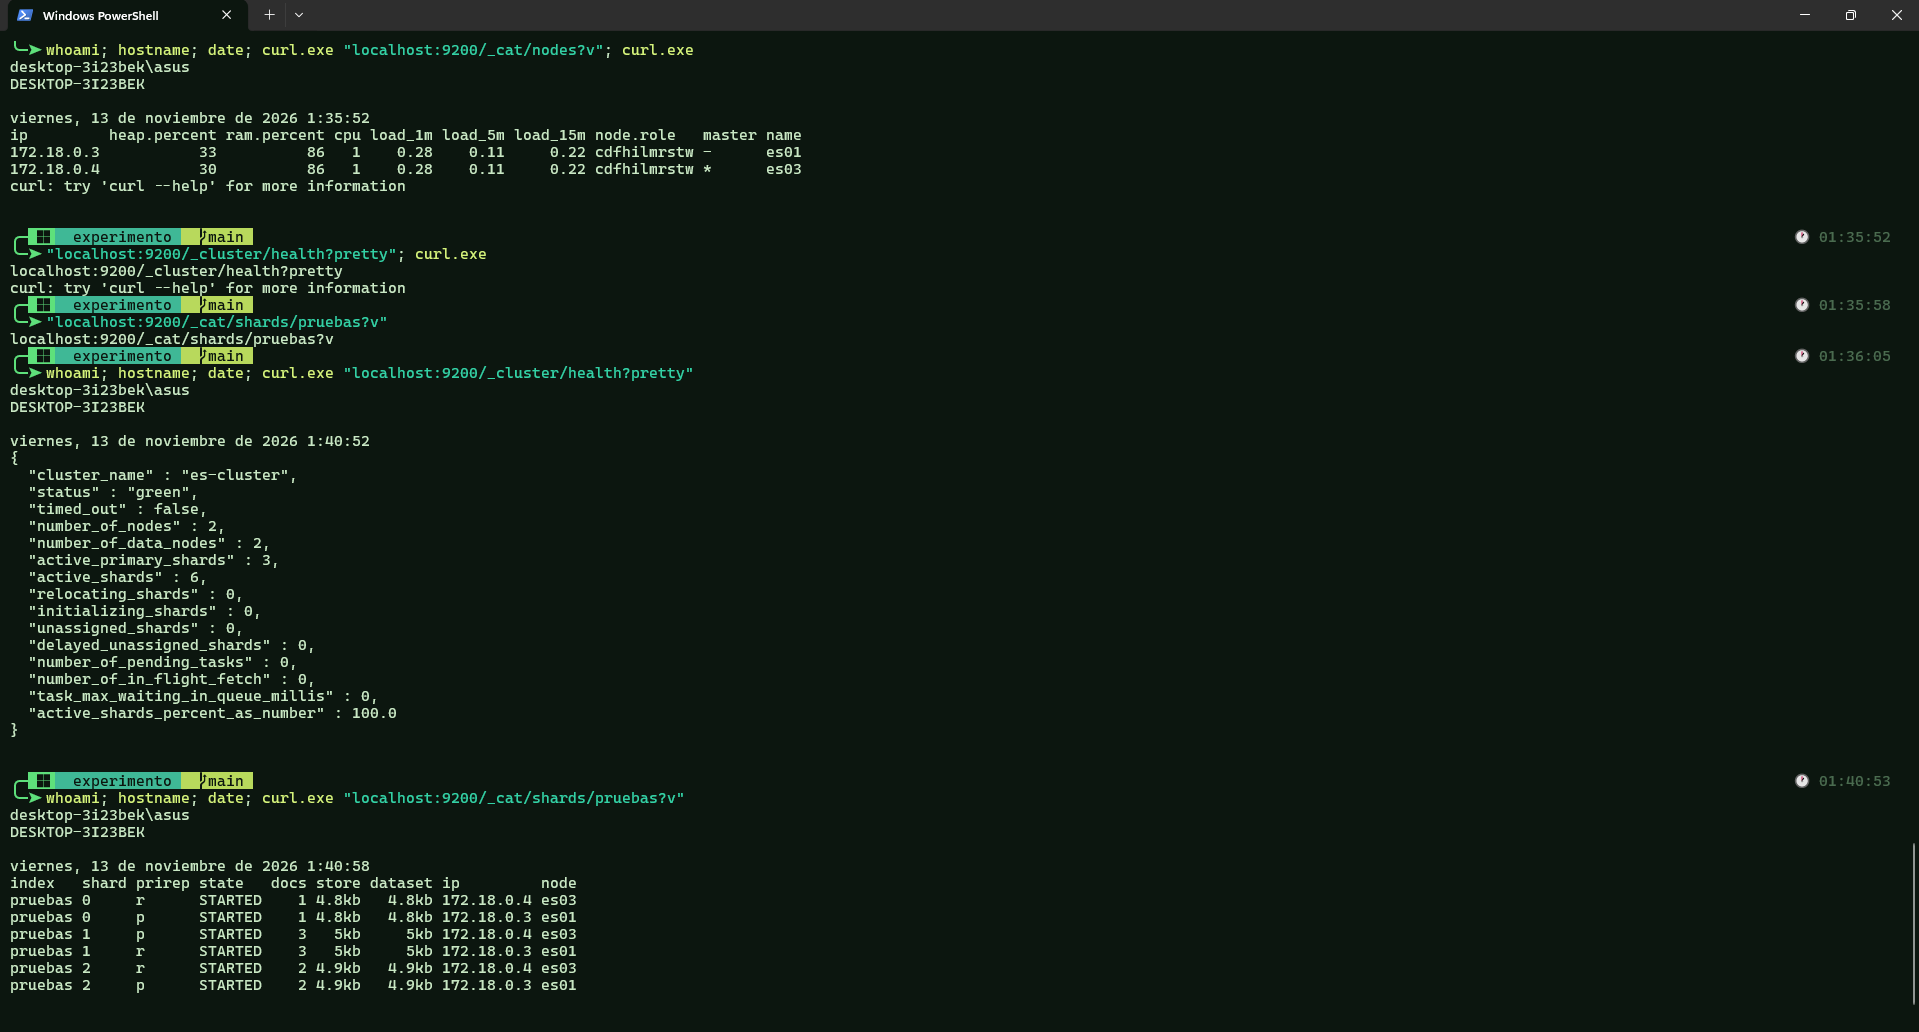
\includegraphics[width=0.92\textwidth]{figuras/captura_03_caida_nodo.png}
    }{
        \fbox{\parbox[c][4cm][c]{0.92\textwidth}{\centering Agregar captura en \texttt{figuras/captura\_03\_caida\_nodo.png} (caída de \texttt{es02}).}}
    }
    \caption{Estado del clúster tras la caída del nodo \texttt{es02} (captura propia).}
    \label{fig:caida}
\end{figure}

\noindent\textbf{Interpretación:} La continuidad del estado \textit{green} y la ausencia de shards sin asignar muestran que el clúster pudo reorganizar las copias disponibles para conservar el servicio. Este comportamiento refleja mecanismos de tolerancia a fallos basados en replicación y gestión del clúster \cite{elastic_resilience,elastic_discovery}.

\subsection{Recuperación del nodo}
Al reiniciar \texttt{es02}, el nodo se reincorporó al clúster (3 nodos activos) y las réplicas se redistribuyeron, volviendo a ocupar nodos distintos según la asignación mostrada por \texttt{\_cat/shards}. Los shards permanecieron en estado \texttt{STARTED} y se conservaron los mismos conteos de documentos.

\begin{figure}[H]
    \centering
    \IfFileExists{figuras/captura_04_recuperacion.png}{
        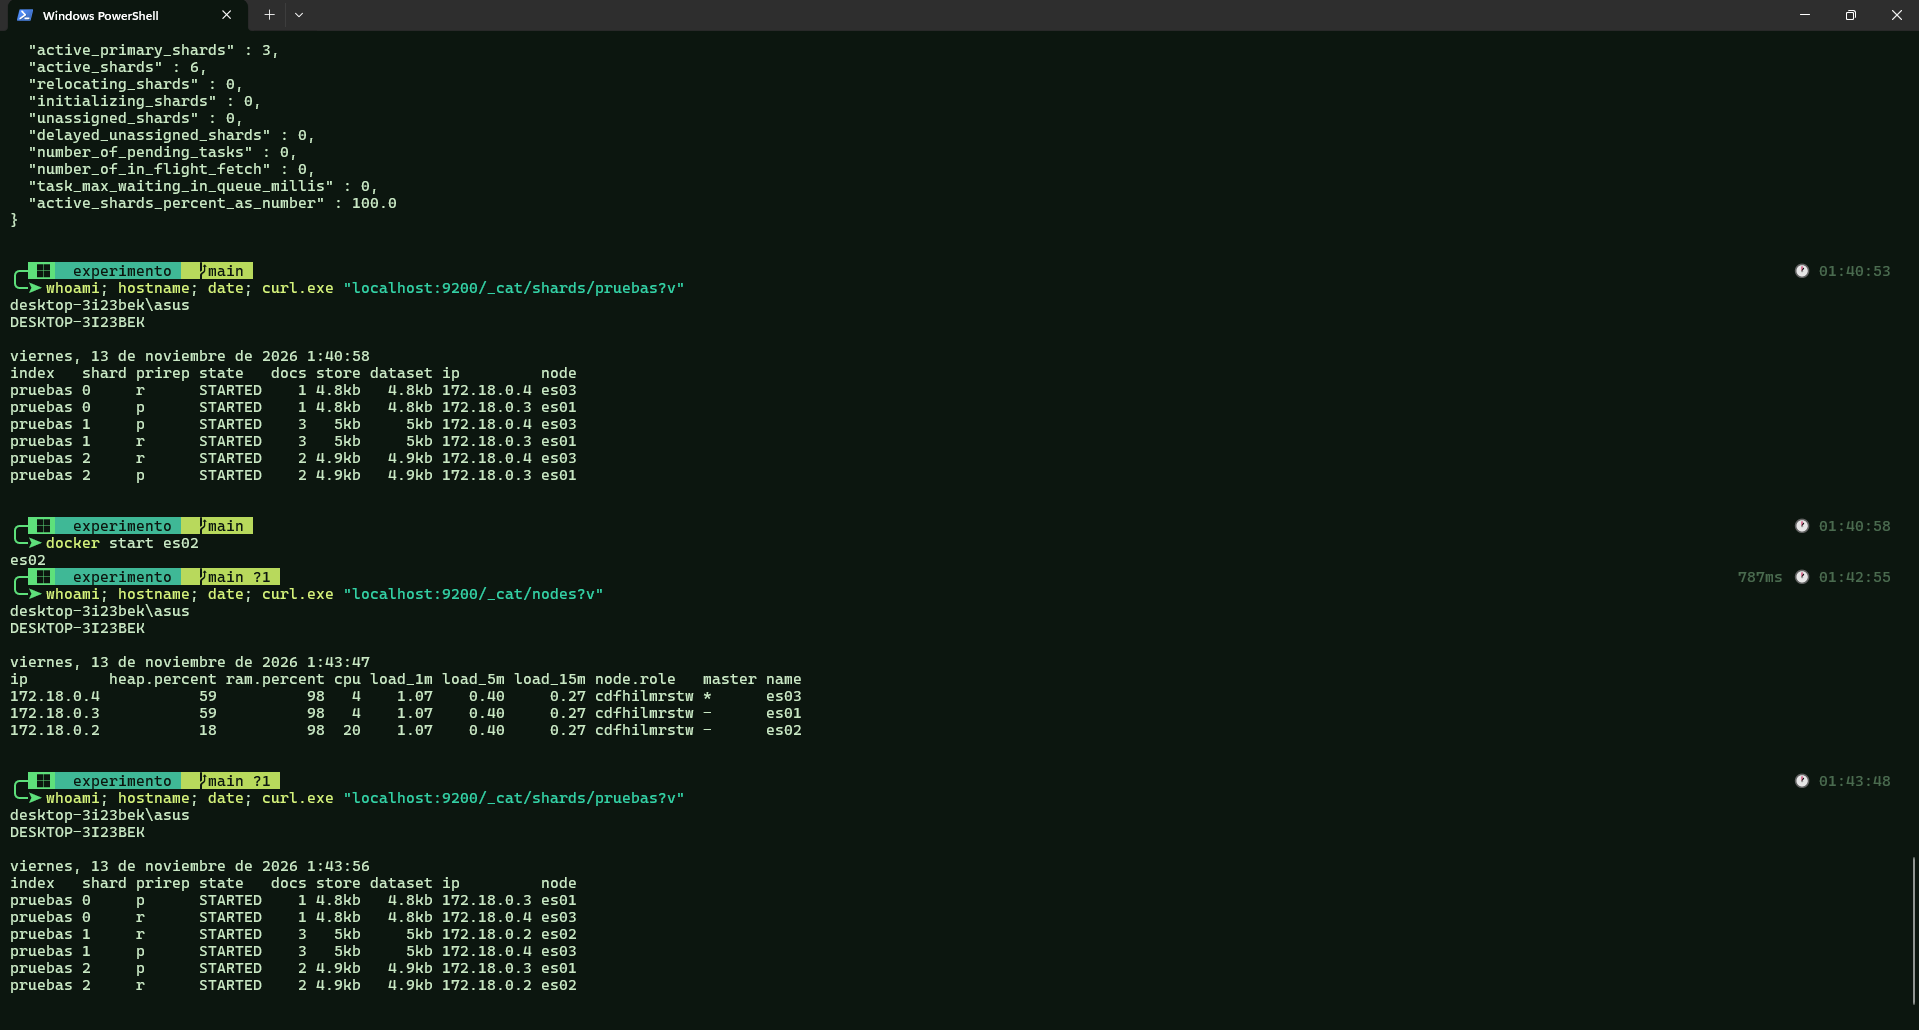
\includegraphics[width=0.92\textwidth]{figuras/captura_04_recuperacion.png}
    }{
        \fbox{\parbox[c][4cm][c]{0.92\textwidth}{\centering Agregar captura en \texttt{figuras/captura\_04\_recuperacion.png} (recuperación de \texttt{es02}).}}
    }
    \caption{Recuperación y redistribución de shards tras reiniciar \texttt{es02} (captura propia).}
    \label{fig:recuperacion}
\end{figure}

\noindent\textbf{Interpretación:} La reincorporación del nodo permitió restablecer la distribución y la redundancia del clúster sin pérdida observable de datos en la prueba. Esto confirma la importancia de las réplicas y los procesos de recuperación para la disponibilidad del sistema \cite{elastic_nodes_shards,elastic_resilience}.

% ===================== EJEMPLOS ENTORNO =====================
\section{Ejemplos del entorno del estudiante}

\subsection{Ejemplo 1: [Completar: nombre del sistema observado]}
% Reemplazar con un sistema real que uses o conozcas (p. ej. SGA UTEQ, banca móvil, WhatsApp).
\textbf{Situación observada:} [Completar: describe una situación concreta observada por ti (caída del servicio, demora en actualización, mensaje tardío, saldo que tardó en reflejarse, etc.)].\\
\textbf{Relación con la Unidad 1:} [Completar: relaciona la situación con conceptos como transparencia de fallos, consistencia eventual, disponibilidad, replicación, comunicación asíncrona o tolerancia a fallos].

\subsection{Ejemplo 2: [Completar: nombre del sistema observado]}
\textbf{Situación observada:} [Completar: describe otra situación concreta observada por ti].\\
\textbf{Relación con la Unidad 1:} [Completar: relaciona la situación con un concepto de la Unidad 1 y justifica brevemente].

% ===================== COMPARATIVO =====================
\section{Análisis comparativo: Elasticsearch vs. Apache Solr}

La Tabla~\ref{tab:comparativo} compara Elasticsearch y Apache Solr (SolrCloud) utilizando criterios de la Unidad 1. La comparación se apoya en estudios académicos \cite{deniz-2023,feraru-2026,unger-2023,lu-2026,cheresharov-2026,calderon-2023} y en documentación técnica oficial \cite{elastic_distributed_architecture,elastic_nodes_shards,elastic_read_write,elastic_discovery,elastic_resilience,solr_shards_indexing,solr_distributed_requests,solr_recoveries}.

\begin{table}[H]
\centering
\caption{Comparación entre Elasticsearch y Apache Solr (SolrCloud)}
\label{tab:comparativo}
\small
\renewcommand{\arraystretch}{1.25}
\begin{tabular}{|p{3.2cm}|p{5.5cm}|p{5.5cm}|}
\hline
\textbf{Criterio (Unidad 1)} & \textbf{Elasticsearch} & \textbf{Apache Solr (SolrCloud)} \\
\hline
Arquitectura y distribución & Clúster de nodos con índices particionados en shards primarios y réplicas; roles de nodos y coordinación distribuida para indexación/búsqueda \cite{elastic_distributed_architecture,elastic_nodes_shards,cheresharov-2026}. & Colecciones distribuidas en shards con réplicas; coordinación de clúster y liderazgo de shard para gestionar actualizaciones y consultas \cite{solr_shards_indexing,solr_distributed_requests}. \\
\hline
Modelos de comunicación & Modelo cliente-servidor vía API HTTP/REST; comunicación interna entre nodos mediante la capa de transporte para descubrimiento, coordinación y replicación \cite{elastic_distributed_architecture,elastic_read_write,elastic_discovery}. & Modelo cliente-servidor vía HTTP/API; distribución y enrutamiento de solicitudes en el clúster, con coordinación entre nodos y componentes de gestión del clúster \cite{solr_distributed_requests,solr_shards_indexing}. \\
\hline
Replicación y consistencia (CAP/PACELC) & Escrituras dirigidas al shard primario y propagadas a réplicas; los compromisos de consistencia, disponibilidad y latencia dependen de la configuración y del estado del clúster \cite{elastic_read_write,elastic_resilience}. & Réplicas de shard con tipos NRT, TLOG y PULL que implican distintos compromisos entre actualización, capacidad de liderazgo, latencia y recuperación \cite{solr_shards_indexing,solr_recoveries}. \\
\hline
Tolerancia a fallos y recuperación & Descubrimiento de nodos, elección de maestro, replicación y reasignación/recuperación de shards ante fallos; en el experimento el clúster mantuvo shards activos tras la caída de un nodo \cite{elastic_discovery,elastic_resilience,elastic_nodes_shards}. & Liderazgo de shard, replicación y mecanismos de recuperación; la tolerancia a fallos depende del tipo y número de réplicas y de la coordinación del clúster. Incidentes de coordinación/liderazgo (p. ej. SOLR-7844) muestran riesgos a considerar \cite{solr_shards_indexing,solr_recoveries,solr_jira_7844}. \\
\hline
Rendimiento y evidencia comparativa & El desempeño depende de configuración y carga; se reporta uso en escenarios de búsqueda/analítica distribuida \cite{cheresharov-2026,feraru-2026,calderon-2023}. & Estudios y casos reportan buen desempeño y confiabilidad en búsqueda/indexación; comparaciones directas muestran resultados variables según escenario y configuración \cite{deniz-2023,unger-2023,lu-2026}. \\
\hline
\end{tabular}
\end{table}

\subsection{Discusión comparativa}
Elasticsearch y SolrCloud comparten una base conceptual similar: ambos distribuyen índices en shards y utilizan réplicas para soportar consultas y fallos. Sin embargo, difieren en la forma de gestionar ciertos aspectos operativos y en los mecanismos disponibles para balancear consistencia, disponibilidad y rendimiento. La evidencia experimental mostró que Elasticsearch puede mantener la disponibilidad de los datos ante la caída de un nodo cuando existen réplicas asignadas correctamente. Por su parte, SolrCloud ofrece opciones explícitas de tipos de réplica (NRT, TLOG, PULL), lo que permite ajustar el comportamiento de indexación y recuperación según las necesidades \cite{solr_shards_indexing,solr_recoveries}.

Los estudios comparativos sugieren que no existe un ganador absoluto: el rendimiento relativo depende del conjunto de datos, la configuración, el hardware y el tipo de consulta \cite{deniz-2023,feraru-2026}. Por ello, la selección entre Elasticsearch y Solr debe considerar no solo velocidad, sino también modelo de operación, tolerancia a fallos, consistencia requerida y capacidades de administración.

% ===================== POSTURA CRÍTICA =====================
\section{Postura crítica}

\subsection{Fortalezas}
Elasticsearch presenta fortalezas importantes como sistema distribuido: escalabilidad horizontal mediante nodos y shards, replicación para disponibilidad, y una interfaz HTTP/REST que facilita la integración con aplicaciones \cite{elastic_distributed_architecture,elastic_nodes_shards,elastic_read_write}. En la experimentación, el clúster mantuvo la disponibilidad de los shards tras la caída de un nodo, lo que evidencia en la práctica el valor de la replicación y la reasignación automática. Además, existe un ecosistema y documentación amplia para su despliegue y observación \cite{calderon-2023,elastic_resilience}.

\subsection{Limitaciones y compromisos (trade-offs)}
El uso de Elasticsearch implica compromisos propios de los sistemas distribuidos. La configuración de shards, réplicas y nodos maestros influye en la resiliencia y el rendimiento: una configuración inadecuada puede afectar la disponibilidad o la recuperación ante fallos \cite{elastic_nodes_shards,elastic_resilience}. Asimismo, la coordinación necesaria para escribir y replicar datos introduce costos de latencia y complejidad operativa \cite{elastic_read_write}. Frente a particiones o fallos de componentes de coordinación, la disponibilidad puede verse comprometida, como lo ilustra el incidente de Elastic Cloud de 2019 \cite{elastic_cloud_incident_2019}. En comparación, SolrCloud también enfrenta compromisos, pero los hace más explícitos en la elección de tipos de réplica y en su dependencia de mecanismos de coordinación \cite{solr_shards_indexing,solr_recoveries}.

\subsection{Contextos donde no sería la mejor opción}
Elasticsearch no sería la mejor opción cuando se requiere un sistema transaccional relacional con garantías ACID tradicionales como requisito principal, cuando el volumen de datos es pequeño y no justifica la complejidad operativa de un clúster distribuido, o cuando las restricciones de recursos impiden sostener múltiples nodos y réplicas. En escenarios donde se prioricen configuraciones específicas de replicación/liderazgo o una integración particular con el ecosistema de Solr, Apache Solr podría ser una alternativa más adecuada \cite{deniz-2023,solr_shards_indexing}.

% ===================== CONCLUSIONES =====================
\section{Conclusiones}

\begin{enumerate}
    \item La experimentación mostró que un clúster de Elasticsearch con réplicas puede mantener el estado \textit{green} y conservar los shards activos ante la caída de un nodo, gracias a la reasignación de copias entre los nodos disponibles.
    \item Elasticsearch y Apache Solr comparten principios de distribución (shards y réplicas), pero presentan diferencias en sus mecanismos de coordinación y en las opciones de configuración (por ejemplo, los tipos de réplica en SolrCloud), lo que implica compromisos distintos entre consistencia, disponibilidad, latencia y recuperación \cite{elastic_read_write,solr_shards_indexing,solr_recoveries}.
    \item La tolerancia a fallos no depende únicamente de contar con réplicas: también influyen la elección de nodos maestros/líderes, la coordinación del clúster y la correcta configuración, como se observó en la práctica y en incidentes documentados \cite{elastic_discovery,elastic_resilience,elastic_cloud_incident_2019,solr_jira_7844}.
    \item La elección entre Elasticsearch y Solr debe basarse en el contexto de uso, los requisitos no funcionales y la evidencia disponible; las comparaciones de rendimiento aportan criterios útiles, pero no reemplazan el análisis de arquitectura y operación distribuida \cite{deniz-2023,unger-2023,feraru-2026}.
\end{enumerate}

% ===================== DECLARACIÓN IA =====================
\section{Declaración de uso de inteligencia artificial}

\textbf{Herramienta:} Claude (Anthropic).\\
\textbf{Uso:} La IA me ayudó a mejorar la redacción, organizar el contenido y escribir el código en LaTeX. También me apoyó en la traducción de los artículos, la documentación utilizada y en la realización del experimento, guiándome con el uso de comandos en la terminal y resolviendo dudas durante el proceso.\\
\textbf{Verificación:} Se revisaron todos los DOI uno por uno con ayuda de IA para traducir y comprender mejor los artículos. También se consultó documentación oficial de las herramientas utilizadas para entender mejor los conceptos y mejorar la elaboración del documento.\\[4pt]

% ===================== REFERENCIAS =====================
\printbibliography[heading=bibintoc,title={Referencias}]

% ===================== ANEXOS =====================
\appendix

\section{Esquema inicial a mano de la arquitectura}
\label{anexo:esquema}
\begin{figure}[H]
    \centering
    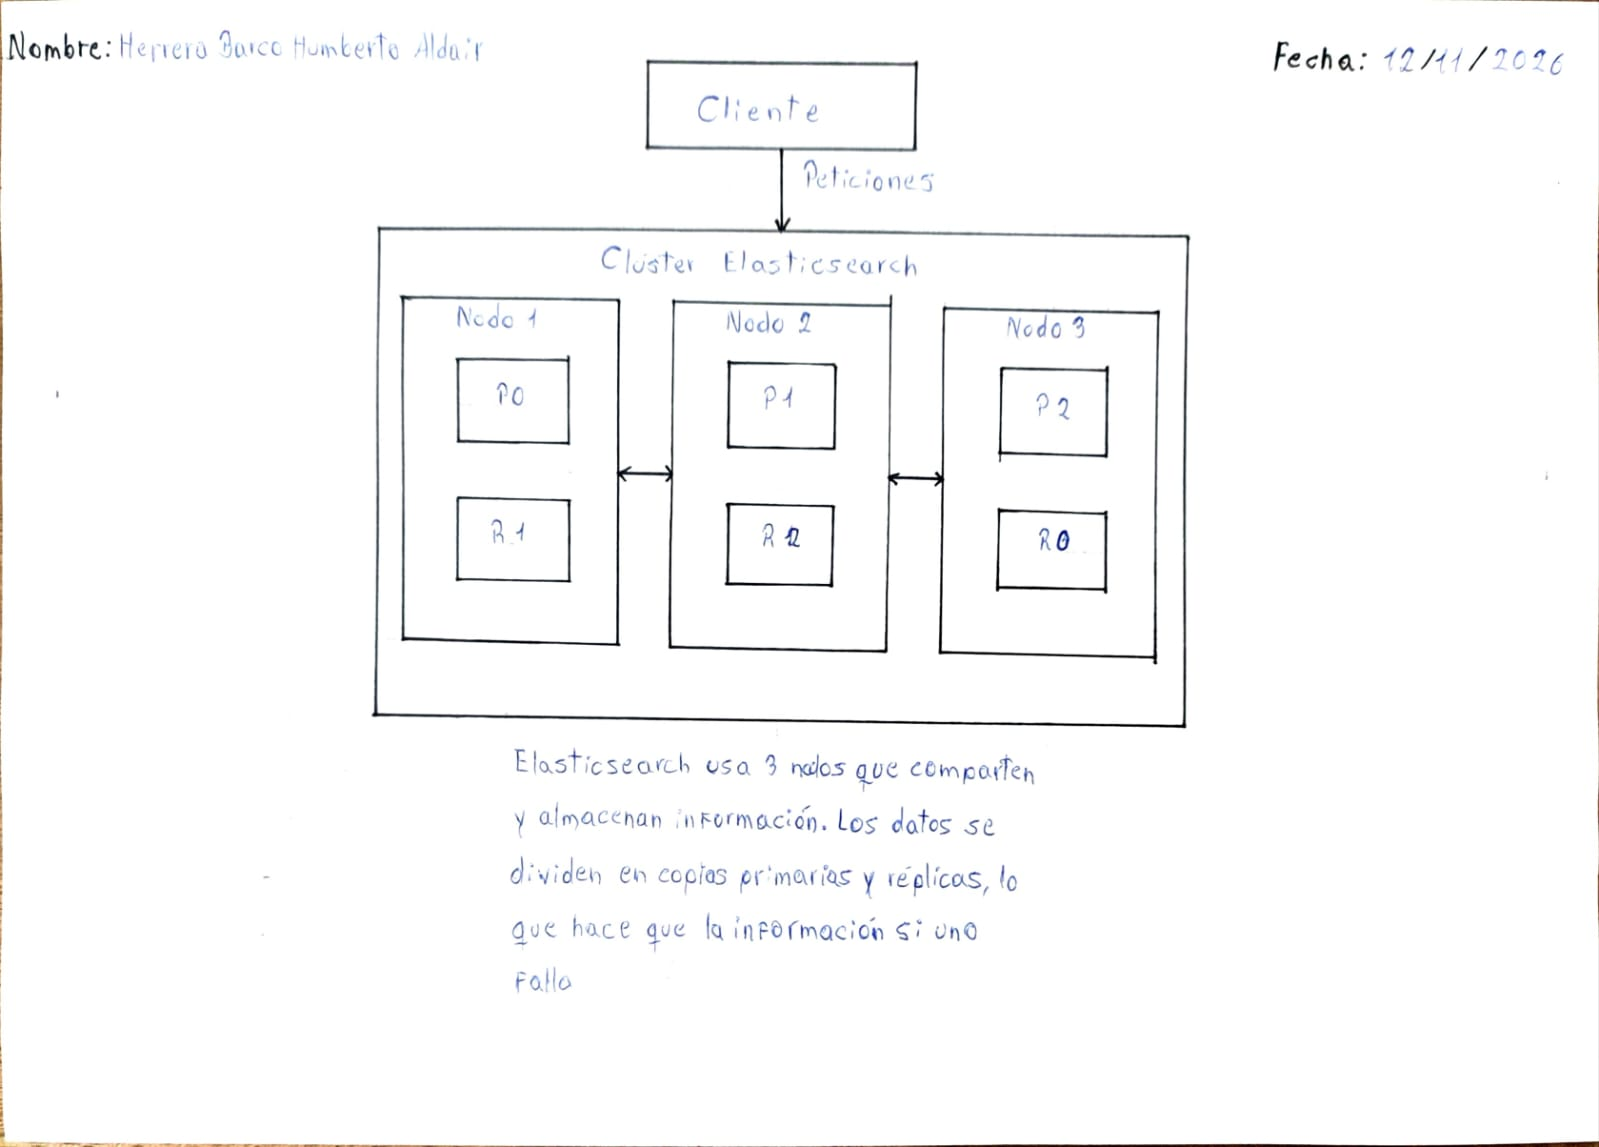
\includegraphics[width=0.85\textwidth]{figuras/anexo_a_esquema_mano.jpeg}
    \caption{Esquema inicial a mano de la arquitectura del clúster (elaboración propia).}
\end{figure}
\noindent\textit{Nota: verificar que en la imagen se aprecien nombre y fecha, según los requisitos de la actividad.}

\section{Capturas de lectura de las fuentes}
\label{anexo:fuentes}

Las siguientes capturas corresponden a fragmentos de los artículos citados en el informe. Cada imagen incluye el pasaje subrayado/anotado y el número de página visible en el PDF.

\subsection{Fuente 1: Comparación de Elasticsearch y Apache Solr \cite{deniz-2023}}
\begin{figure}[H]
    \centering
    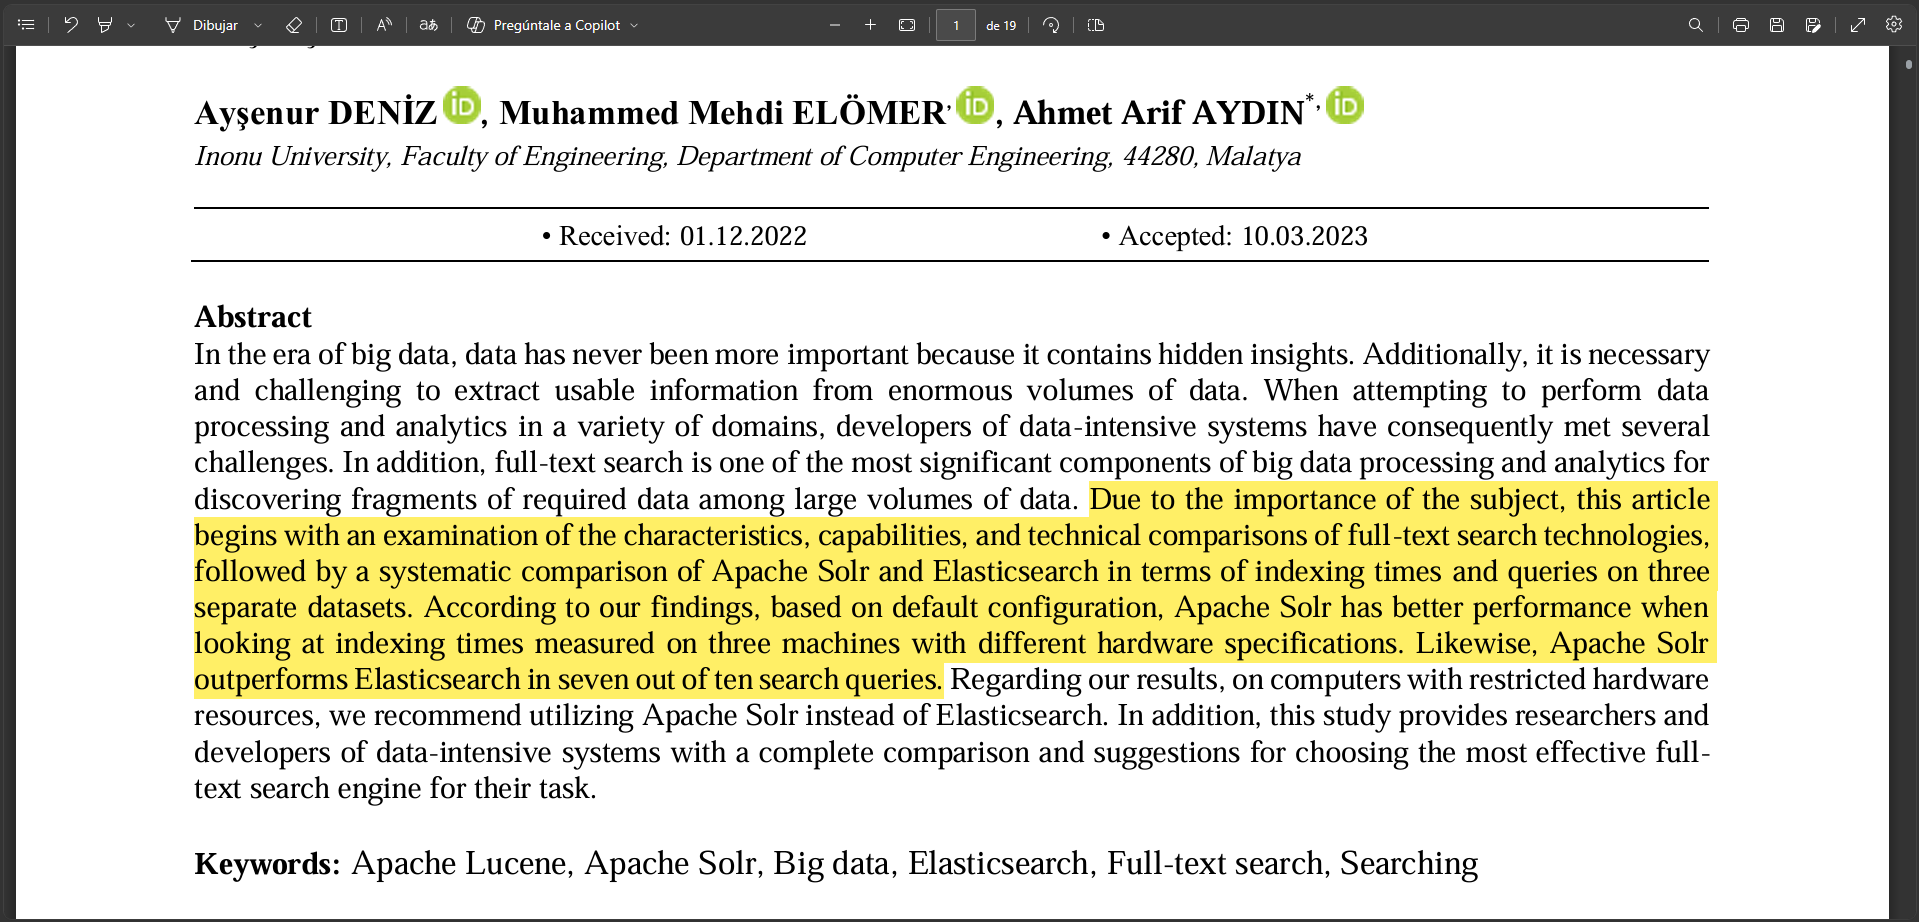
\includegraphics[width=0.92\textwidth]{figuras/anexo_b_deniz_2023.png}
    \caption{Lectura anotada de Deniz et al. (2023), utilizada como respaldo de la comparación entre Elasticsearch y Apache Solr \cite{deniz-2023}.}
\end{figure}

\subsection{Fuente 2: Plataforma distribuida con Elasticsearch y Kafka \cite{calderon-2023}}
\begin{figure}[H]
    \centering
    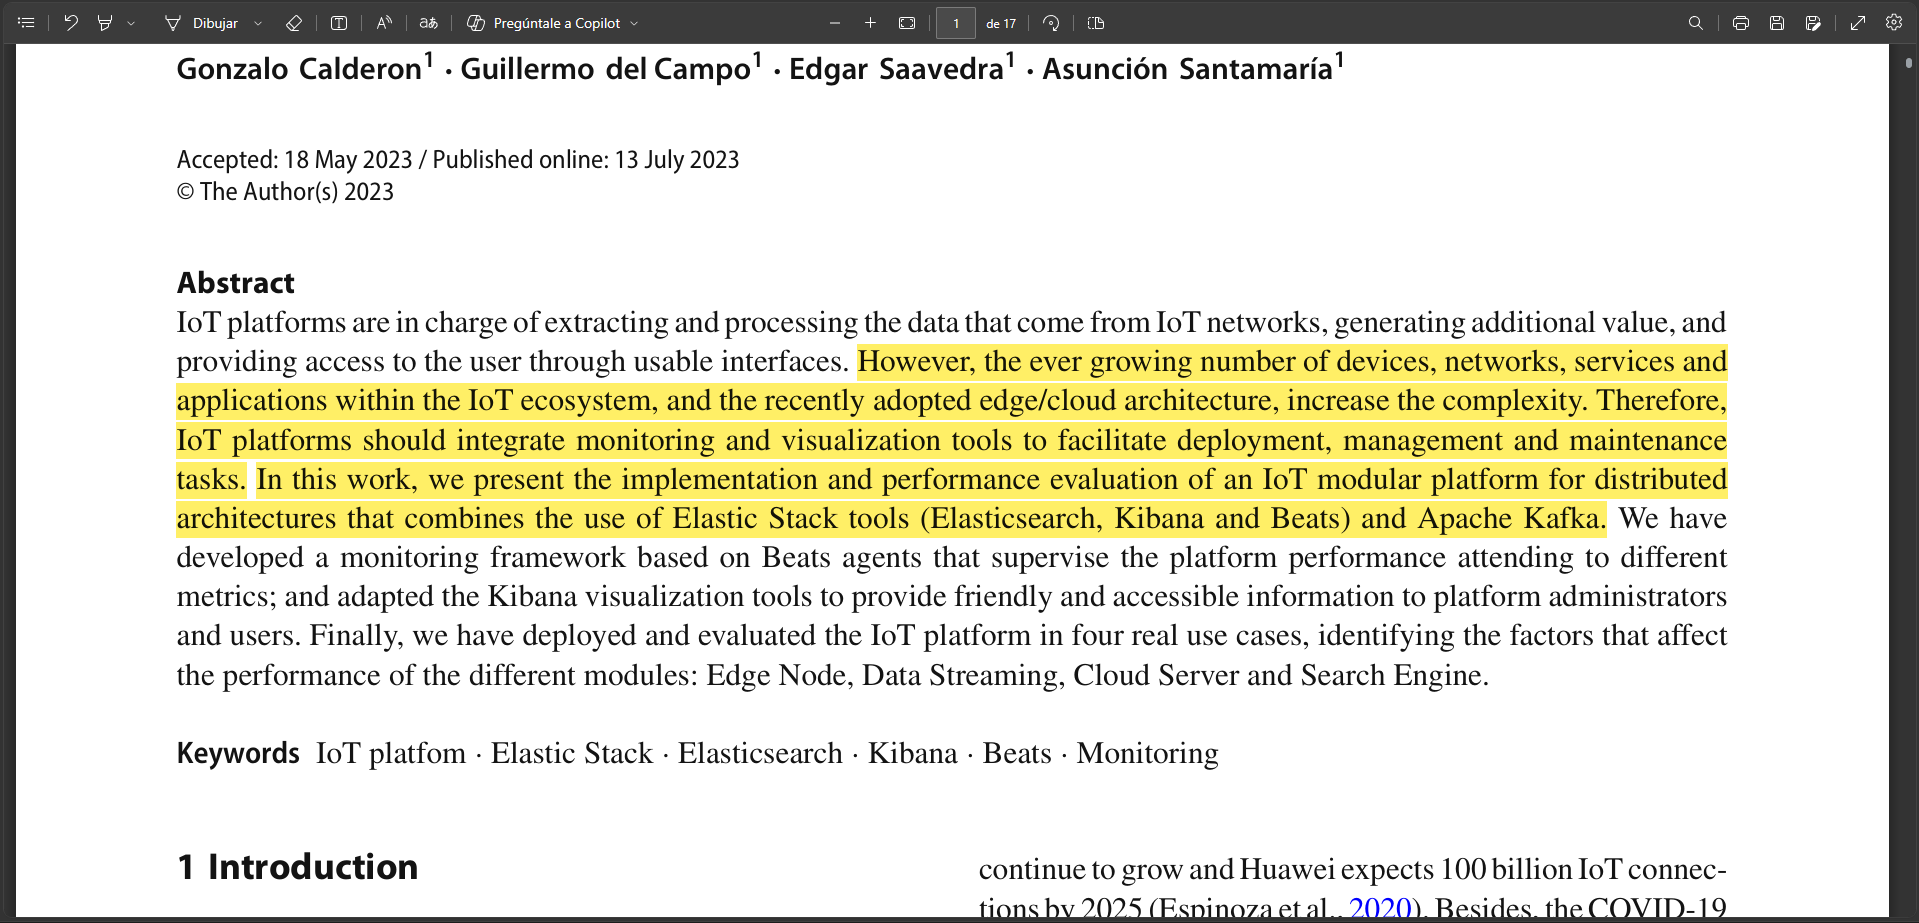
\includegraphics[width=0.92\textwidth]{figuras/anexo_b_calderon_2023.png}
    \caption{Lectura anotada de Calderon et al. (2023), utilizada como respaldo del uso de Elasticsearch en arquitecturas distribuidas \cite{calderon-2023}.}
\end{figure}

\subsection{Fuente 3: Uso de Solr y evaluación de rendimiento \cite{unger-2023}}
\begin{figure}[H]
    \centering
    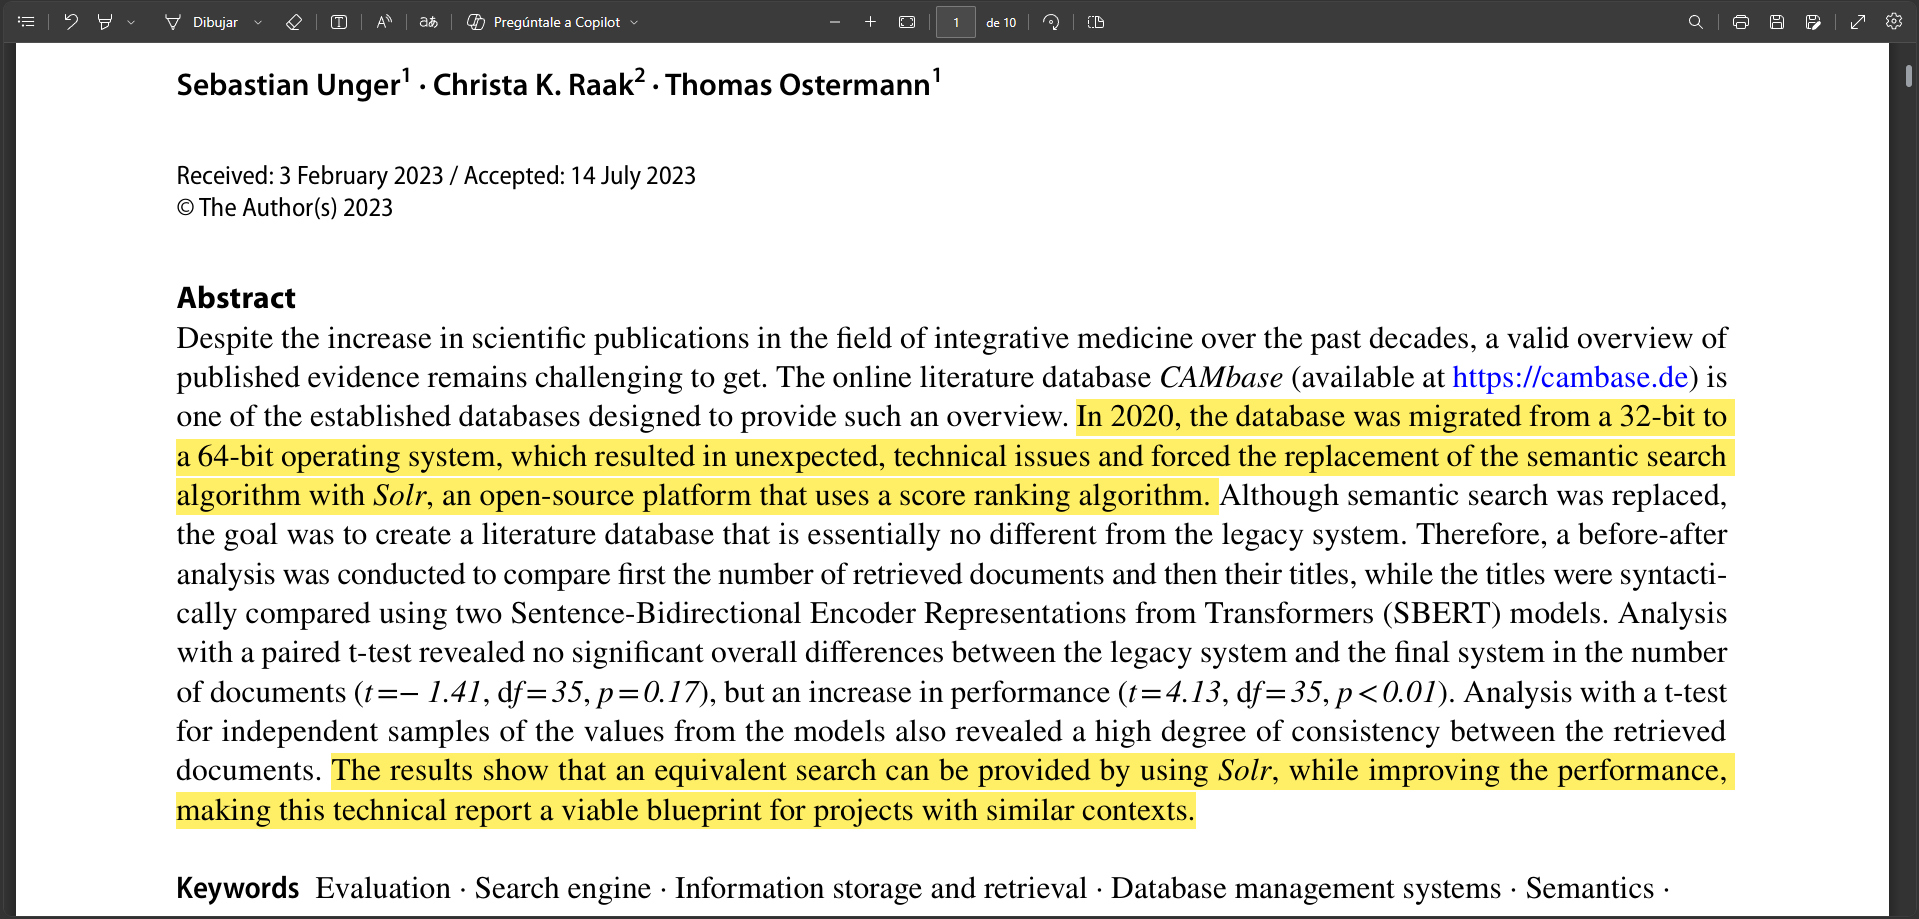
\includegraphics[width=0.92\textwidth]{figuras/anexo_b_unger_2023.png}
    \caption{Lectura anotada de Unger et al. (2023), utilizada como respaldo del uso y rendimiento de Apache Solr \cite{unger-2023}.}
\end{figure}

\end{document}
